\documentclass[11pt]{article}
\usepackage[utf8]{inputenc}
\usepackage[T1]{fontenc}
\usepackage{amsmath}
\usepackage{multicol}
\usepackage{geometry}
\usepackage{tikz}
\usetikzlibrary{shapes.geometric, arrows.meta}
\usepackage{enumitem}
\usepackage{xcolor}
\usepackage{titlesec}

% Configurações de layout
\geometry{a4paper, left=1cm, right=1cm, top=0.5cm, bottom=1.2cm}
\setlength{\columnseprule}{0.4pt}
\setlength{\baselineskip}{1.0\baselineskip}

% Cores para títulos
\titleformat{\section}{\normalfont\Large\bfseries\color{blue}}{\thesection}{1em}{}
\titleformat{\subsection}{\normalfont\large\bfseries\color{red}}{\thesubsection}{1em}{}
\titleformat{\subsubsection}{\normalfont\normalsize\bfseries\color{black}}{\thesubsubsection}{1em}{}

\title{\textcolor{blue}{Revisão: Plano Cartesiano, Funções do 1\textdegree e 2\textdegree grau.}}
\author{Professor: Jefferson}
\date{}

\begin{document}

\maketitle
\vspace{-1cm}

\begin{center}
\large{Nome: \underline{\hspace{8cm}} \quad Turma: \underline{\hspace{3cm}}}
\end{center}

\begin{multicols}{2}

\section*{1. Plano Cartesiano}
Sistema de coordenadas com dois eixos perpendiculares:
\begin{itemize}
    \item Eixo horizontal (x): abscissas
    \item Eixo vertical (y): ordenadas
    \item Origem: ponto (0,0)
    \item Quadrantes: 4 regiões numeradas anti-horário
\end{itemize}

\begin{center}
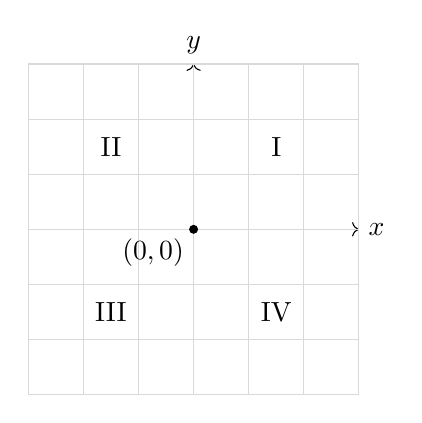
\begin{tikzpicture}[scale=0.7]
    \draw[->] (-3,0) -- (3,0) node[right]{$x$};
    \draw[->] (0,-3) -- (0,3) node[above]{$y$};
    \draw[gray!30] (-3,-3) grid (3,3);
    \filldraw (0,0) circle (2pt) node[below left]{$(0,0)$};
    \node at (1.5,1.5) {I};
    \node at (-1.5,1.5) {II};
    \node at (-1.5,-1.5) {III};
    \node at (1.5,-1.5) {IV};
\end{tikzpicture}
\end{center}

\section*{2. Função do 1º Grau}
$f(x) = ax + b$

\subsection*{Características}
\begin{itemize}
    \item Gráfico: reta
    \item Raiz: $x = -\frac{b}{a}$
    \item $a>0$: crescente \quad $a<0$: decrescente
    \item $b$: intercepto no eixo y
\end{itemize}

\begin{center}
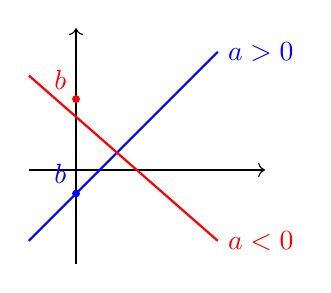
\begin{tikzpicture}[scale=0.6]
    \draw[->] (-1,0) -- (4,0);
    \draw[->] (0,-2) -- (0,3);
    \draw[blue, thick] (-1,-1.5) -- (3,2.5) node[right]{$a>0$};
    \draw[red, thick] (-1,2) -- (3,-1.5) node[right]{$a<0$};
    \filldraw[blue] (0,-0.5) circle (2pt) node[above left]{$b$};
    \filldraw[red] (0,1.5) circle (2pt) node[above left]{$b$};
\end{tikzpicture}
\end{center}

\section*{3. Função do 2º Grau}
$f(x) = ax^2 + bx + c$

\subsection*{Características}
\begin{itemize}
    \item Gráfico: parábola
    \item Concavidade: $a>0$ (cima) \quad $a<0$ (baixo)
    \item Vértice: $V=\left(-\frac{b}{2a}, -\frac{\Delta}{4a}\right)$
    \item Raízes: $x = \frac{-b \pm \sqrt{\Delta}}{2a}$, $\Delta=b^2-4ac$
\end{itemize}

\begin{center}
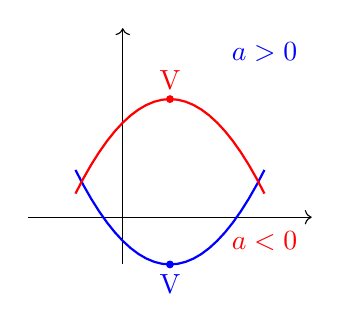
\begin{tikzpicture}[scale=0.6]
    \draw[->] (-2,0) -- (4,0);
    \draw[->] (0,-1) -- (0,4);
    \draw[blue, thick] plot[domain=-1:3] (\x, {0.5*\x*\x - \x - 0.5});
    \draw[red, thick] plot[domain=-1:3] (\x, {-0.5*\x*\x + \x + 2});
    \filldraw[blue] (1,-1) circle (2pt) node[below]{V};
    \filldraw[red] (1,2.5) circle (2pt) node[above]{V};
    \node at (3,3.5) [blue] {$a>0$};
    \node at (3,-0.5) [red] {$a<0$};
\end{tikzpicture}
\end{center}

\subsection*{Vértice e Eixo de Simetria}
\begin{itemize}
    \item $x_v = -\frac{b}{2a}$ (eixo de simetria)
    \item $y_v = f(x_v)$ (valor máximo/mínimo)
\end{itemize}

\section*{4. Comparação dos Gráficos}

\begin{center}
\begin{tabular}{|l|l|l|}
\hline
 & 1º Grau & 2º Grau \\
\hline
Forma & Reta & Parábola \\
Raízes & 1 & 0, 1 ou 2 \\
Vértice & Não tem & Ponto de máximo/mínimo \\
Variação & Constante & Variável \\
\hline
\end{tabular}
\end{center}

\begin{center}
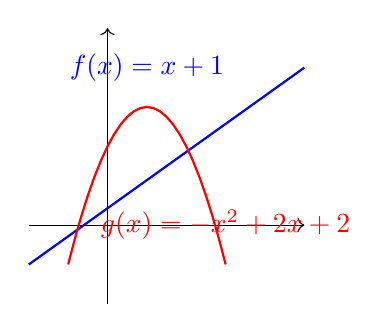
\begin{tikzpicture}[scale=0.5]
    \draw[->] (-2,0) -- (5,0);
    \draw[->] (0,-2) -- (0,5);
    \draw[blue, thick] (-2,-1) -- (5,4);
    \draw[red, thick] plot[domain=-1:3] (\x, {-\x*\x + 2*\x + 2});
    \node at (1,4) [blue] {$f(x)=x+1$};
    \node at (3,0) [red] {$g(x)=-x^2+2x+2$};
\end{tikzpicture}
\end{center}

\section*{5. Análise Completa da Parábola}

\subsection*{Exemplo: $f(x) = x^2 - 4x + 3$}
\begin{enumerate}
    \item Concavidade: $a=1>0$ (para cima)
    \item Raízes: $x^2-4x+3=0 \Rightarrow x=1$ ou $x=3$
    \item Vértice: $x_v = \frac{4}{2}=2$, $y_v = -1$ \\ $V(2,-1)$
    \item Intercepto y: $(0,3)$
\end{enumerate}

\begin{center}
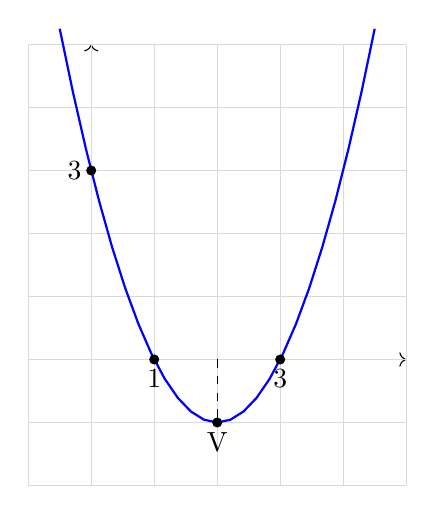
\begin{tikzpicture}[scale=0.8]
    \draw[->] (-1,0) -- (5,0);
    \draw[->] (0,-2) -- (0,5);
    \draw[gray!30] (-1,-2) grid (5,5);
    \draw[blue, thick] plot[domain=-0.5:4.5] (\x, {\x*\x -4*\x +3});
    \filldraw (1,0) circle (2pt) node[below]{1};
    \filldraw (3,0) circle (2pt) node[below]{3};
    \filldraw (0,3) circle (2pt) node[left]{3};
    \filldraw (2,-1) circle (2pt) node[below]{V};
    \draw[dashed] (2,0) -- (2,-1);
\end{tikzpicture}
\end{center}

\section*{6. Exercícios}

\subsection*{Identificação}
1. Classifique e caracterize:
\begin{enumerate}[label=\alph*)]
    \item $f(x) = 3x - 6$
    \item $g(x) = -x^2 + 4$
    \item $h(x) = x^2 - 6x + 9$
\end{enumerate}

\subsection*{Gráficos}
2. Esboce os gráficos de:
\begin{enumerate}[label=\alph*)]
    \item $y = -2x + 3$
    \item $y = x^2 - 4$
    \item $y = -x^2 + 2x$
\end{enumerate}

\subsection*{Análise}
3. Para $f(x) = x^2 - 5x + 6$, determine:
\begin{enumerate}[label=\alph*)]
    \item Concavidade
    \item Raízes
    \item Vértice
    \item Estudo do sinal
\end{enumerate}

\subsection*{Aplicações}
4. O lucro de uma empresa é dado por $L(x) = -x^2 + 80x - 700$, onde $x$ são unidades vendidas.
\begin{enumerate}[label=\alph*)]
    \item Quantas unidades para lucro máximo?
    \item Qual o lucro máximo?
    \item Entre que valores de $x$ há lucro?
\end{enumerate}

\section*{7. Análise de Gráficos (Exercícios Visuais)}

\subsection*{Instruções}
Analise cada gráfico e responda às perguntas correspondentes. Considere as características como raízes, vértice, crescimento, decrescimento, concavidade etc.

\begin{center}
\textbf{Gráfico 1: Função do 1º Grau}
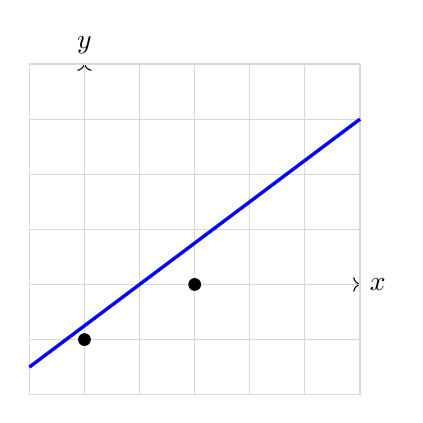
\begin{tikzpicture}[scale=0.7]
    \draw[->] (-1,0) -- (5,0) node[right]{$x$};
    \draw[->] (0,-2) -- (0,4) node[above]{$y$};
    \draw[gray!30] (-1,-2) grid (5,4);
    \draw[blue, very thick] (-1,-1.5) -- (5,3);
    \filldraw (2,0) circle (3pt);
    \filldraw (0,-1) circle (3pt);
\end{tikzpicture}

\vspace{0.5cm}
\textbf{Perguntas:}
\begin{enumerate}[label=\alph*)]
    \item Qual o coeficiente linear (ponto onde corta o eixo y)?
    \item Qual a raiz da função?
    \item A função é crescente ou decrescente?
\end{enumerate}
\end{center}

\begin{center}
\textbf{Gráfico 2: Função do 2º Grau}
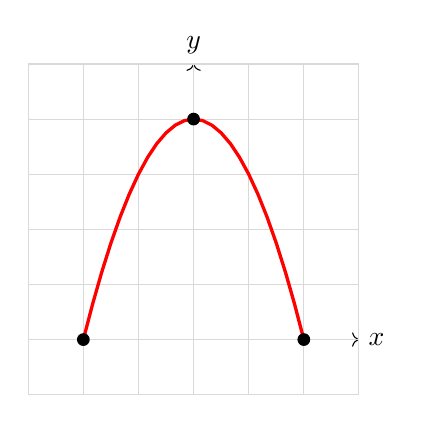
\begin{tikzpicture}[scale=0.7]
    \draw[->] (-3,0) -- (3,0) node[right]{$x$};
    \draw[->] (0,-1) -- (0,5) node[above]{$y$};
    \draw[gray!30] (-3,-1) grid (3,5);
    \draw[red, very thick] plot[domain=-2:2] (\x, {-\x*\x + 4});
    \filldraw (-2,0) circle (3pt);
    \filldraw (2,0) circle (3pt);
    \filldraw (0,4) circle (3pt);
\end{tikzpicture}

\vspace{0.5cm}
\textbf{Perguntas:}
\begin{enumerate}[label=\alph*)]
    \item Quais são as raízes da função?
    \item Qual as coordenadas do vértice?
    \item A concavidade é para cima ou para baixo?
\end{enumerate}
\end{center}

\begin{center}
\textbf{Gráfico 4: Função Quadrática com Vértice Fora da Origem}
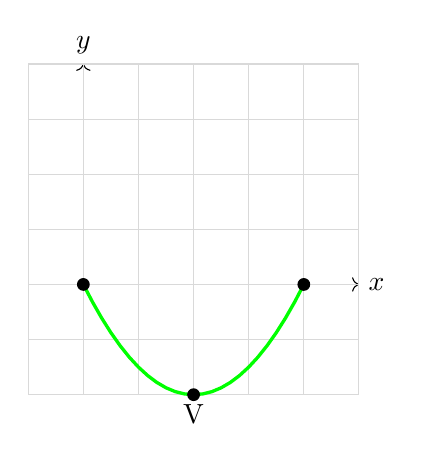
\begin{tikzpicture}[scale=0.7]
    \draw[->] (-1,0) -- (5,0) node[right]{$x$};
    \draw[->] (0,-2) -- (0,4) node[above]{$y$};
    \draw[gray!30] (-1,-2) grid (5,4);
    \draw[green, very thick] plot[domain=0:4] (\x, {0.5*\x*\x - 2*\x});
    \filldraw (0,0) circle (3pt);
    \filldraw (4,0) circle (3pt);
    \filldraw (2,-2) circle (3pt) node[below]{V};
\end{tikzpicture}

\vspace{0.5cm}
\textbf{Perguntas:}
\begin{enumerate}[label=\alph*)]
    \item Qual o valor mínimo da função?
    \item Em que intervalo a função é decrescente?
    \item Qual o valor de $f(3)$?
\end{enumerate}
\end{center}

\end{multicols}

\end{document}
